\section{Dataset Selection and Characteristics}
\label{sec:dataset}

This section outlines our dataset selection criteria and analyzes the characteristics of the chosen datasets for evaluating clustering algorithms.

\subsection{Dataset Selection}

To evaluate clustering algorithms, we selected three datasets with diverse characteristics in size, attribute types, class distribution, and missing data patterns. This diversity allows for a comprehensive analysis of algorithm performance under varying conditions.

The datasets vary in size, including a small dataset (Hepatitis), a medium-sized dataset (Vowel), and a large dataset (Mushroom), enabling an assessment of scalability and computational efficiency. They also include diverse attribute types: nominal, numerical, and mixed, ensuring the algorithms are tested across different data representations.

Class distribution was another consideration. Although clustering is unsupervised, class distributions serve as baselines for validating cluster quality. We included a balanced dataset (Vowel), a slightly imbalanced one (Mushroom), and a heavily imbalanced one (Hepatitis). Lastly, missing data patterns were addressed, with Hepatitis containing missing values to test robustness, while Vowel and Mushroom datasets are complete, allowing performance comparisons under ideal conditions.


% \subsection{Dataset Selection}
% To evaluate the performance of clustering algorithms, we selected three datasets with diverse characteristics in size,
% attribute types, class distribution, and missing data patterns. This diversity ensures a comprehensive analysis of algorithm efficiency under varying conditions.

% % \subsection{Dataset Selection}
% % In this project, we aimed to select three datasets that offer substantial variability across different aspects to evaluate the performance of various clustering algorithms, such as K-Means, G-Means, OPTICS, gs-FCM, etc.

% % The criteria for dataset selection were centered around diversity in dataset size, attribute types, class distribution, and missing data patterns. These factors allowed us to thoroughly analyze the efficiency and effectiveness of each clustering algorithm under different scenarios.

% \paragraph{Dataset size variation} 
% To examine the scalability of the clustering algorithms, we selected one small dataset (Hepatitis), one medium-sized dataset (Vowel), and one large dataset (Mushroom). This setup enables us to assess the computational requirements and clustering performance of the algorithms across varying dataset sizes.

% \paragraph{Attribute type diversity} 
% We chose datasets with diverse attribute types, including nominal, numerical, and mixed attributes. This ensures that the clustering algorithms are evaluated for their ability to handle varying data representations and preprocessing requirements.

% \paragraph{Class distribution} 
% Although clustering is an unsupervised learning task, the class distributions of the datasets can serve as a baseline for validating the quality of clusters. We included one dataset with balanced classes (Vowel), one with slightly imbalanced classes (Mushroom), and one with a heavily imbalanced distribution (Hepatitis).

% \paragraph{Missing data patterns} 
% We considered datasets with varying levels of missing data. The Hepatitis dataset contains missing values, challenging the algorithms to handle incomplete information, while the Vowel and Mushroom datasets are complete, ensuring a comparison of clustering performance in the absence of missing data.

\subsection{Dataset Characteristics}

The Hepatitis dataset includes 155 instances with a mix of 13 nominal and 6 numerical attributes. It represents a binary classification problem (survive vs. die), but the classes are imbalanced, with the majority class comprising 79.35\% of the instances. Approximately 6.01\% of the values are missing. 

The Mushroom dataset consists of 8,124 instances with 22 nominal attributes. It represents a binary classification problem (edible vs. poisonous) with nearly balanced classes and contains no missing values. 

The Vowel dataset contains 990 instances with 3 nominal and 10 numerical attributes. It represents a multi-class classification problem with 11 balanced classes and no missing values. 


% \begin{table*}[h]
% \centering
% \begin{tabular}{|l|c|c|c|}
% \hline
% \textbf{Dataset}      & \textbf{Mushroom}                & \textbf{Hepatitis}              & \textbf{Vowel}                  \\ \hline
% \textbf{Instances}    & 8,124                           & 155                             & 990                             \\ \hline
% \textbf{Attributes}   & 22 nominal                      & 13 nominal, 6 numerical         & 3 nominal, 10 numerical         \\ \hline
% \textbf{Classification Type} & Binary (edible vs. poisonous) & Binary (survive vs. die)        & Multi-Class (11 classes)        \\ \hline
% \textbf{Class Balance} & Nearly balanced                 & Imbalanced (79.35\% majority)   & Balanced                        \\ \hline
% \textbf{Missing Values} & None                            & 6.01\%                          & None                            \\ \hline
% \end{tabular}
% \caption{Characteristics of the Mushroom, Hepatitis, and Vowel datasets.}
% \label{tab:dataset_characteristics}
% \end{table*}


% \subsection{Dataset Characteristics}

% \begin{itemize}
%     \item \textbf{Mushroom Dataset}
%     \begin{itemize}
%         \item 8,124 instances
%         \item 22 nominal attributes
%         \item Binary classification (edible vs. poisonous)
%         \item Nearly balanced classes
%         \item No missing values
%     \end{itemize}
    
%     \item \textbf{Hepatitis Dataset}
%     \begin{itemize}
%         \item 155 instances
%         \item Mixed attribute types (13 nominal and 6 numerical)
%         \item Binary classification (survive vs. die)
%         \item Imbalanced classes (79.35\% majority class)
%         \item 6.01\% missing values
%     \end{itemize}

%     \item \textbf{Vowel Dataset}
%     \begin{itemize}
%         \item 990 instances
%         \item Mixed attribute types (3 nominal and 10 numerical)
%         \item Multi-Class classification (11 classes)
%         \item Balanced classes
%         \item No missing values
%     \end{itemize}
% \end{itemize}

\subsection{Selection Criteria}
We selected the Hepatitis, Mushroom, and Vowel datasets to provide complementary characteristics for evaluating clustering algorithms. Our selection criteria focused on:

\begin{itemize}
    \item \textbf{Dataset size variation} (small, medium, large)
    \item \textbf{Attribute type diversity} (nominal, numerical, mixed)
\end{itemize}



% \subsection{Dataset Selection and Characteristics}
% \label{subsec:dataset}

% This section outlines our dataset selection criteria and analyzes the characteristics of the chosen datasets.

% \subsubsection{Dataset Selection}
% In this project, we aimed to select two datasets that offer substantial variability across different aspects to evaluate the performance of Support Vector Machine (SVM) and k-Nearest Neighbors (KNN) algorithms.
% The criteria for dataset selection were centered around having one dataset that is small and another that is large, allowing us to analyze both the efficiency and effectiveness of these models across differing dataset sizes.
% \paragraph{Smaller datasets} 
% \paragraph{Larger datasets} 

% \paragraph{Attribute types} We wanted to assess the models' ability to handle datasets with different types of attributes.
% For this purpose, we wanted to select one dataset with primarily nominal attributes and another with numerical features.
% This allows us to evaluate how well each algorithm handles the representation and processing of different data types.
% \paragraph{Class distribution} By choosing one dataset with a balanced distribution and another with a notable class imbalance, we aim to observe how SVM and KNN, particularly with reduction, perform in scenarios where the data is skewed.
% \paragraph{Missing data} Lastly, we prioritized finding datasets with varying levels of missing data to examine how effectively the algorithms manage incomplete information.

% Based on these criteria, we selected the Hepatitis and Mushroom datasets, as they provide the most distinct and complementary combination for our evaluation.
% \subsubsection{Selection Criteria}
% We selected two datasets with contrasting characteristics to evaluate the performance of Support Vector Machine (SVM) and k-Nearest Neighbors (KNN) algorithms across different scenarios. Our selection criteria focused on:

% \begin{itemize}
%     \item Dataset size variation (small vs. large)
%     \item Attribute type diversity (nominal vs. numerical)
%     \item Class distribution (balanced vs. imbalanced)
%     \item Missing data patterns
% \end{itemize}

% A smaller dataset enables rapid experimentation and initial algorithm validation, while a larger dataset allows evaluation of reduction methods' effectiveness, particularly for KNN's storage and computational requirements.

% \subsubsection{Dataset Characteristics}

% \begin{itemize}
%     \item \textbf{Mushroom Dataset}
%     \begin{itemize}
%         \item 8,124 instances
%         \item 22 nominal attributes
%         \item Binary classification (edible vs. poisonous)
%         \item Nearly balanced classes
%     \end{itemize}
    
%     \item \textbf{Hepatitis Dataset}
%     \begin{itemize}
%         \item 155 instances
%         \item Mixed attribute types (13 nominal and 6 numerical)
%         \item Binary classification (survive vs. die)
%         \item Imbalanced classes (79.35\% majority class)
%         \item 6.01\% missing values
%     \end{itemize}

%     \item \textbf{Vowel Dataset}
%     \begin{itemize}
%         \item 990 instances
%         \item Mixed attribute types (3 nominal and 10 numerical)
%         \item Multi-Class classification (11 classes)
%         \item Balanced classes
%         \item No missing values

%     \end{itemize}
% \end{itemize}

% \begin{figure}
%     \centering
%     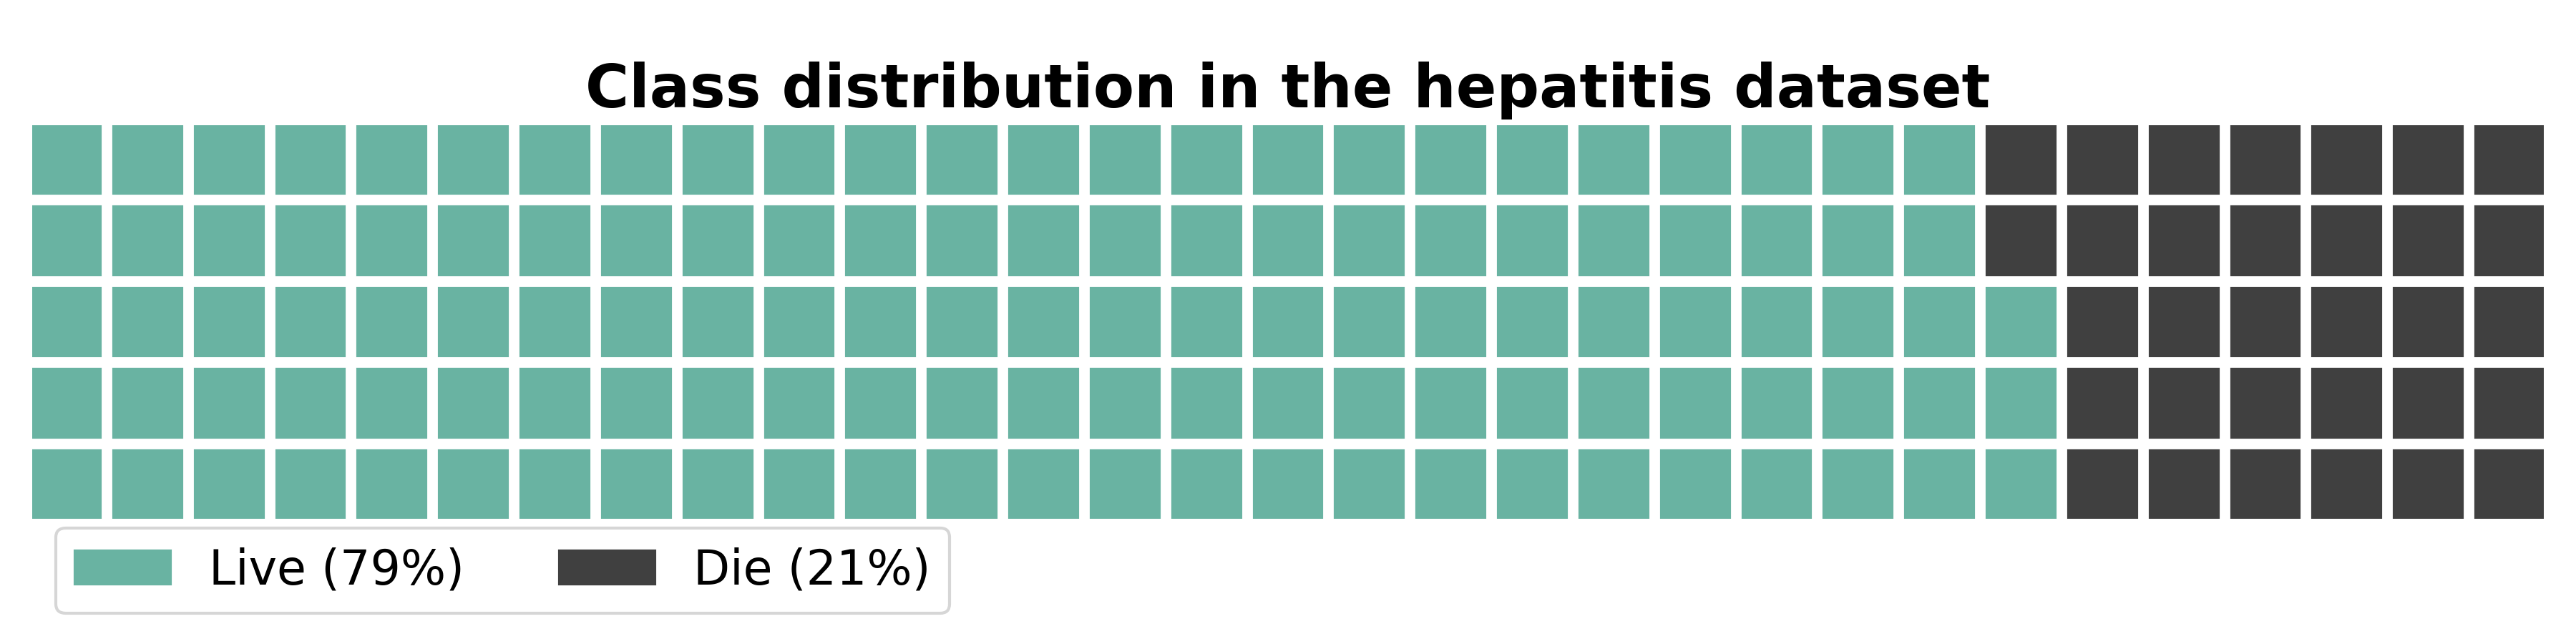
\includegraphics[width=0.45\textwidth]{figures/hepatitis-class-distribution.png}
%     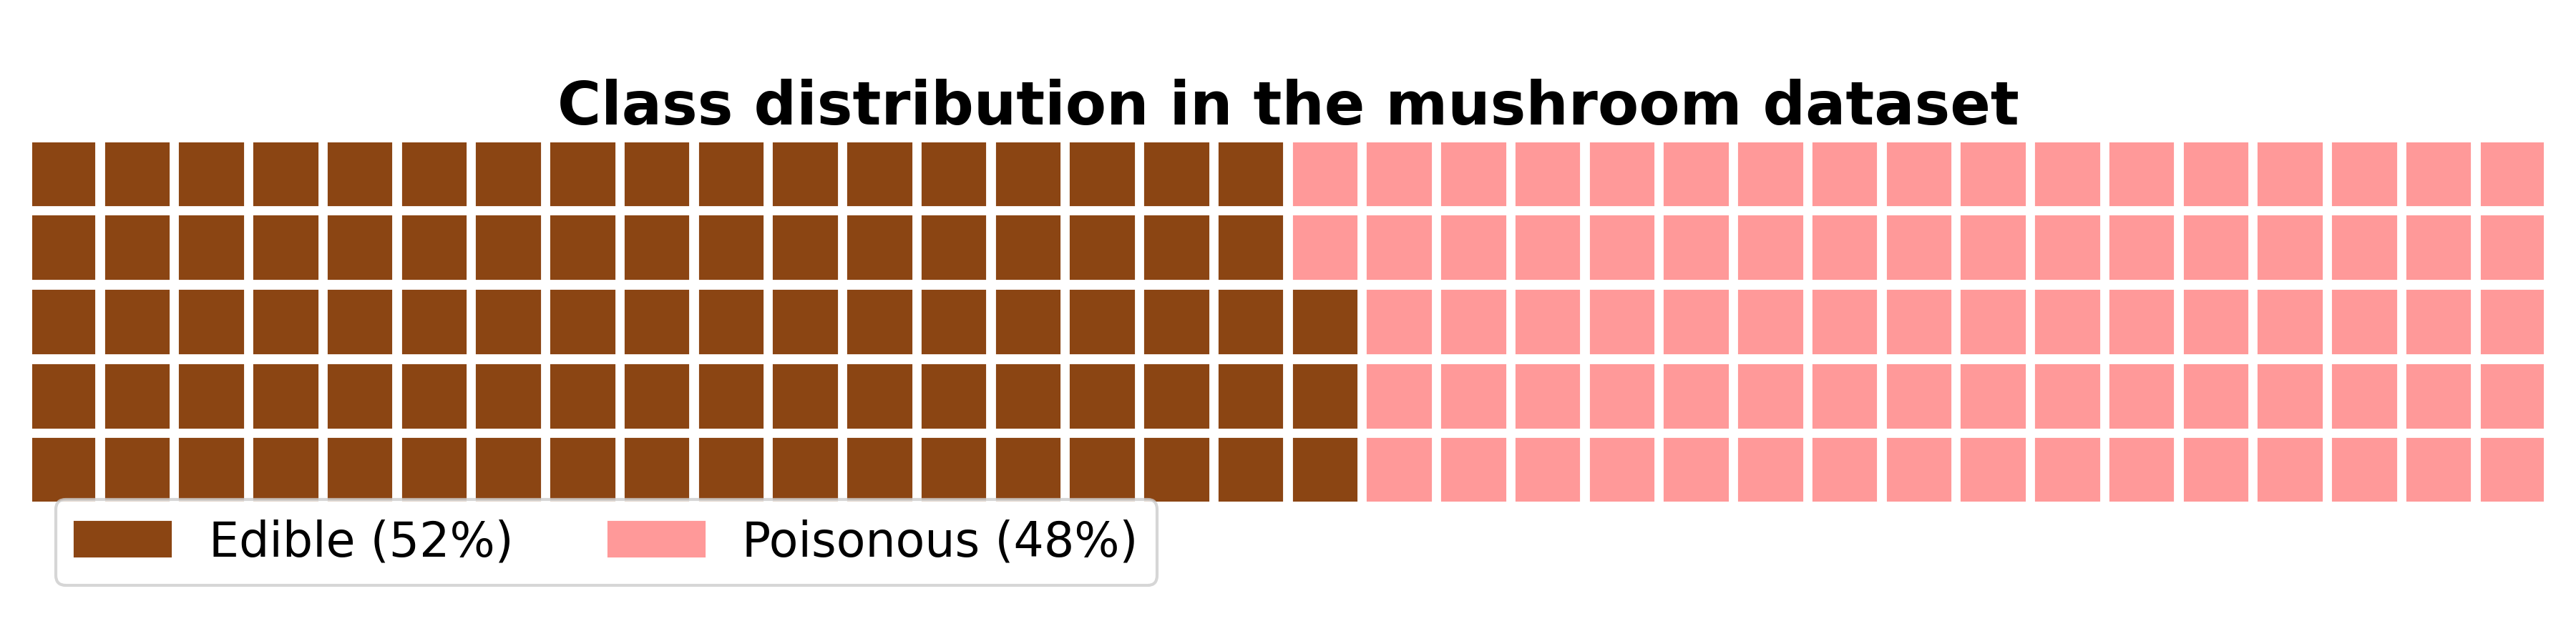
\includegraphics[width=0.45\textwidth]{figures/mushroom-class-distribution.png}
%     \caption{Class distribution comparison between datasets}
%     \label{fig:class-distributions}
% \end{figure}

% These datasets provide complementary characteristics for evaluating our algorithms' performance across different scenarios. The Mushroom dataset challenges the algorithms with its size and categorical nature, while the Hepatitis dataset tests their ability to handle mixed data types and class imbalance.